\documentclass[a4paper,12pt]{article}
\usepackage[utf8]{inputenc}
\usepackage[T2A]{fontenc}
\usepackage[russian,english]{babel}
\usepackage[pdftex]{graphics}
\DeclareGraphicsExtensions{.pdf,.png,.jpg}
\graphicspath{{pictures/}}
\begin{document}
\begin{center}
Санкт-Петербургский государственный политехнический университет
\\Кафедра компьютерных систем и программных технологий
\end{center}
\vspace*{10em plus .6em minus .5em}

\begin{center}
{\LARGEТелекоммуникационные технологии
\\Лабораторная работа №4
\\Аналоговая модуляция}
\end{center}

\vspace*{5em plus .6em minus .5em}
\begin{flushright}
Выполнил:\\студент гр.33501/4\\Корсков Алексей\\Проверила:\\Богач Н.В.
\end{flushright}

\vspace*{15em plus .6em minus .5em}
\begin{center}
{\smallСанкт-Петербург
\\2018}
\end{center}
\pagestyle{empty}
\newpage
\pagestyle{plain}
{\bfseriesЦель}

Изучение амплитудной модуляции/демодуляции сигнала.

{\bfseriesПостановка задачи}

\begin{itemize}
	\item Сгенерировать однотональный сигнал низкой частоты.
	\item Выполнить амплитудную модуляцию (АМ) сигнала по закону $u(t)=(1+MU_mcos(\Omega t))+cos(\omega_0t+\phi_0)$ для различных значений глубины модуляции M. Используйте встроенную функцию
	MatLab ammod.
	\item Получить спектр модулированного сигнала.
	\item Выполнить модуляцию с подавлением несущей $u(t)=MU_mcos(\Omega t)cos(\omega_0 t+\phi_0)$. Получить спектр.
	\item  Выполнить однополосную модуляцию:
		
	$U(t)=U_mcos(\Omega t)cos(\omega_0t+\phi_0)+\frac{U_m}{2}\sum_{n=1}^{N}M_n(cos(\omega_0+\Omega_n)t+\phi_0+\Phi_0)$, положив n=1.
	\item Выполнить синхронное детектирование и получить исходный однополосный сигнал
	\item Рассчитать КПД модуляции
	
	$\eta_AM=\frac{U_m^2M^2/4}{P_U}=\frac{M^2}{M^2+2}$
\end{itemize}

{\bfseriesТеоретическое обоснование}

Модуляция — процесс изменения одного или нескольких параметров модулируемого несущего сигнала при помощи модулирующего сигнала. Амплитудная модуляции -- вид модуляции, при которой изменяемым параметром несущего сигнала является его амплитуда.\\\\
Основными достоинствами амплитудной модуляции являются:
\begin{itemize}
\item узкая ширина спектра АМ сигнала;
\item простота получения модулированных сигналов.\\
\end{itemize}
Недостатками этой модуляции являются:
\begin{itemize}
\item низкая помехоустойчивость;
\item неэффективное использование мощности передатчика.\\
\end{itemize}

Коэффициент полезного действия модуляции определяется по формуле:\\

$\eta_AM=\frac{U_m^2M^2/4}{P_U}=\frac{M^2}{M^2+2}$\\

Модуляция с подавлением несущей частоты - вид модуляции, при которой происходит подавление несущего колебания, что делает КПД модуляции равным 100\%. Модуляция с подавлением несущей выполняется по закону:\\

$U(t)=U_mcos(\Omega t)cos(\omega_0t+\phi_0)+\frac{U_m}{2}\sum_{n=1}^{N}M_n(cos(\omega_0+\Omega_n)t+\phi_0+\Phi_0)$\\
\newpage

{\LargeХод работы}
\begin{enumerate}
{\itemСгенерируем сигнал.
\center{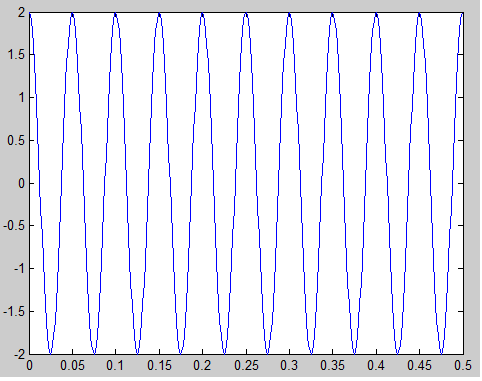
\includegraphics{./pictures/pic1.png} \\ Рис.1 Сигнал}
\\}

{\itemВыполним амплитудную модуляцию, используя функцию ammod.
\center{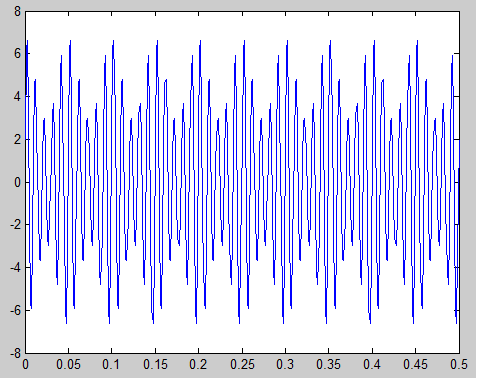
\includegraphics{./pictures/pic2.png} \\ Рис.2 Амплитудная модуляция}
\center{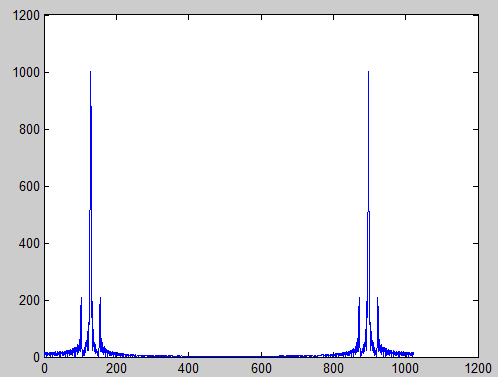
\includegraphics{./pictures/pic3.png} \\ Рис.3 Спектр сигнала}
\\}

{\itemВыполним модуляцию с подавлением несущей.
\center{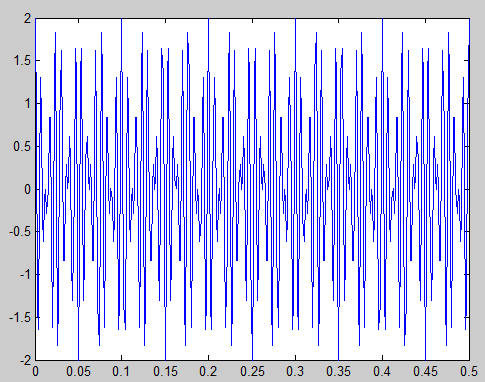
\includegraphics{./pictures/pic4.png} \\ Рис.4 Модуляция с подавлением несущей}
\center{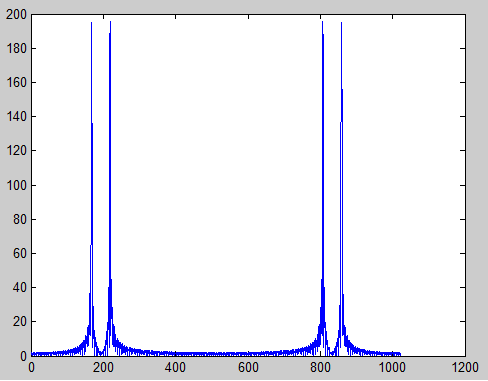
\includegraphics{./pictures/pic5.png} \\ Рис.5 Спектр сигнала}
\\}

{\itemВыполним однополосную модуляцию, используя функцию ssbmod.
\center{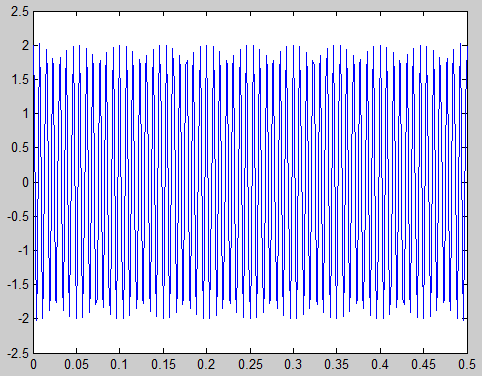
\includegraphics{./pictures/pic6.png} \\ Рис.6 Однополосная модуляция}
\center{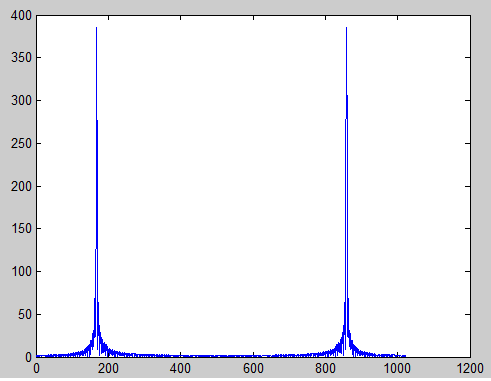
\includegraphics{./pictures/pic7.png} \\ Рис.7 Спектр сигнала}
\\}

{\itemВыполним синхронное детектирование и получим исходный однополосный сигнал.
\center{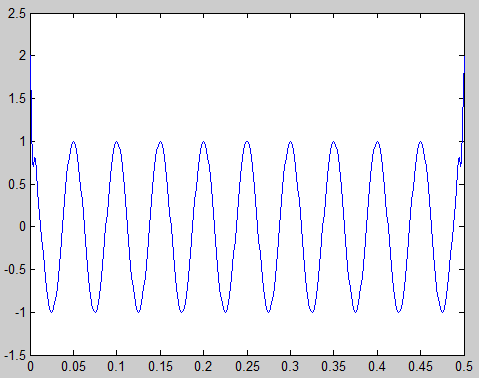
\includegraphics{./pictures/pic8.png} \\ Рис.8 Сигнал после синхронного детектирования}
\center{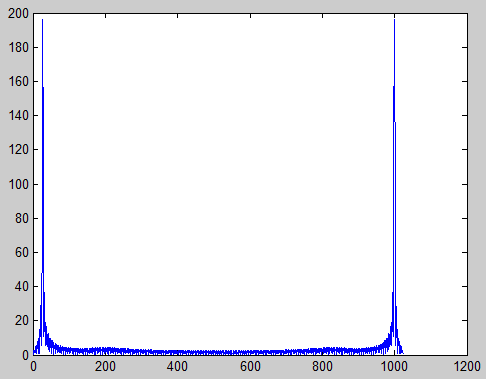
\includegraphics{./pictures/pic9.png} \\ Рис.9 Спектр сигнала}
\\}

{\itemНайдем КПД амплитудной модуляции.
КПД = 0.0196
\\}

{\bfseries\LARGEВывод}

В ходе выполнения лабораторной работы исследована амплитудная модуляция/демодуляция сигнала. Основная мощность передаваемого информационного сигнала намного меньше мощности несущего колебания, поэтому амплитудная модуляция имеет низкий КПД. При подавлении несущей КПД модуляции равно 100\%.

\end{enumerate}
\end{document}
